\section{Ensemble-Methoden}
Oftmals ist der Suchraum für das Problem zu groß, als das es möglich wäre in tolerabler Zeit die optimale Lösung zu finden \cite{laurent1976constructing}. Konstruktionsalgorithmen für Entscheidungsbäume arbeiten aus
diesem Grund auf Basis von Heuristiken um die lokal optimale Teilung zu bestimmen. Im Gegensatz zu diesen Algorithmen versuchen Ensemble-Methoden nicht die beste Lösung, sondern konstruieren eine Menge von Lösungen
unter denen anschließend gewählt wird, was die finale Lösung für ein Problem ist \cite{dietterich2002ensemble}.

\subsection{Voting}
\subsection{Bagging}
\begin{figure}
    \centering
    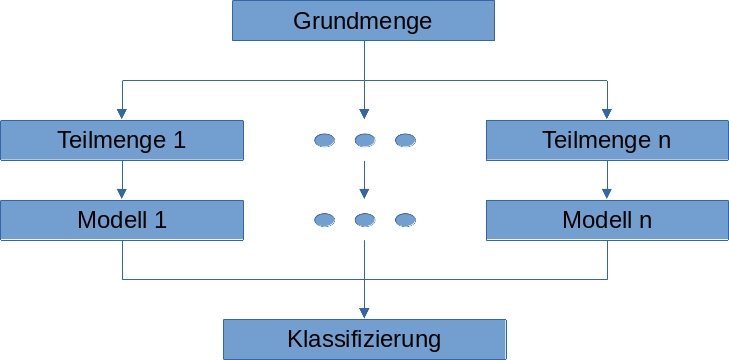
\includegraphics[width=0.6\linewidth]{images/bagging.jpg}
    \caption{Klassifizierungsprozess mit der Bagging-Methode.}
    \label{fig:bagging}
\end{figure}
Bagging ist ein Acronym für \glqq \textbf{B}ootstrap \textbf{agg}regat\textbf{ing}\grqq. Die Idee ist aus einer großen Menge von Trainingsdaten, eine Menge von Mengen von Trainingsdaten zu generieren, folgend mit jedem
dieser Mengen einen Klassifizierer zu trainieren und schließlich alle Klassifizierer, e.g. durch Wählen, zu aggregieren (siehe Abbildung \ref{fig:bagging}) \cite{breiman1996bagging}. Die Methode die dahinter steht nennt
sich \glqq Bootstrap sampling\grqq, welche einen Prozess beschreibt aus einer Grundmenge $m$ mal jeweils $n$ Einträge zu ziehen, die eine Teilmenge bilden \cite{efron1992bootstrap}. Der Name ist folglich aus der Methode
und dem Aggregierungsprozess abgleitet.
\subsection{Random Forest}
Random Forest ist eine Erweiterung der Bagging-Methode. Zusätzlich zu der zufällig ausgewählten Menge an Trainingsdaten wird auch zufällig eine Menge von Features ausgewählt. Auf dieser Basis wird ein Menge von
Entscheidungsbäumen generiert die anschließend aggregiert werden \cite{breiman2001random}.
\subsection{Boosting?}